\ChapterImageStar[cap:caracterizacionGRID]{Caracterización del GRID}{./images/fondo.png}
\label{cap:caracterizacionGRID}
\mbox{}\\
El Grupo de Investigación en Redes, Información y Distribución (\GRID) de la Universidad del Quindío se enmarca en los objetivos misionales de la institución: educación, investigación y extensión. Su propósito central es impulsar el desarrollo a través de proyectos de investigación aplicada, formación académica y transferencia de conocimiento. En particular, el \GRID busca ofrecer servicios tecnológicos avanzados a la comunidad académica, con énfasis en los estudiantes de Ingeniería de Sistemas y Computación, quienes encuentran en este grupo un espacio de formación e innovación en temas de infraestructura, software y tecnologías emergentes.\\
La caracterización del \GRID\@resulta esencial para comprender su estructura, capacidades y necesidades en relación con la adopción de tecnologías de virtualización basadas en contenedores (\VBC). A continuación, se presenta un análisis detallado de los diferentes aspectos que definen el contexto institucional y tecnológico del grupo.

\section{Análisis de stakeholders del GRID}
Con el fin de identificar los actores internos y externos que influyen en el desarrollo de las actividades del grupo, se realizó un análisis de \textit{stakeholders}. Este ejercicio permitió reconocer los diferentes intereses, roles y niveles de influencia que cada actor tiene en relación con la posible implementación de una solución de virtualización por contenedores. Los principales \textit{stakeholders} identificados incluyen: investigadores del grupo, estudiantes de pregrado y posgrado, docentes de la Facultad de Ingeniería, y en un nivel más amplio, la comunidad académica de la Universidad del Quindío.\\
La tabla~\ref{tab:stakeholders} presenta el análisis de los principales interesados en la adopción de tecnologías de virtualización dentro del contexto institucional. Se identifican actores internos y externos, especificando su rol, el tipo de relación con el proyecto, el nivel de impacto esperado, así como su poder de influencia, interés y compromiso frente a la iniciativa. Este análisis permite reconocer que el Grupo de Investigación \GRID constituye el beneficiario principal y el decisor estratégico, mientras que los docentes y estudiantes de Ingeniería de Sistemas representan usuarios clave y finales que validarán la utilidad de la solución en actividades académicas y de investigación. A nivel institucional, el programa de ingeniería de sistemas y computación actúa como facilitador de recursos y lineamientos, mientras que los proveedores de tecnología aportan las herramientas de virtualización requeridas. De forma complementaria, los investigadores externos y otros grupos de investigación pueden beneficiarse indirectamente de los resultados, y el sector empresarial se perfila como un potencial socio estratégico si percibe ventajas competitivas en la solución.
\begin{table}[H]
    \centering
    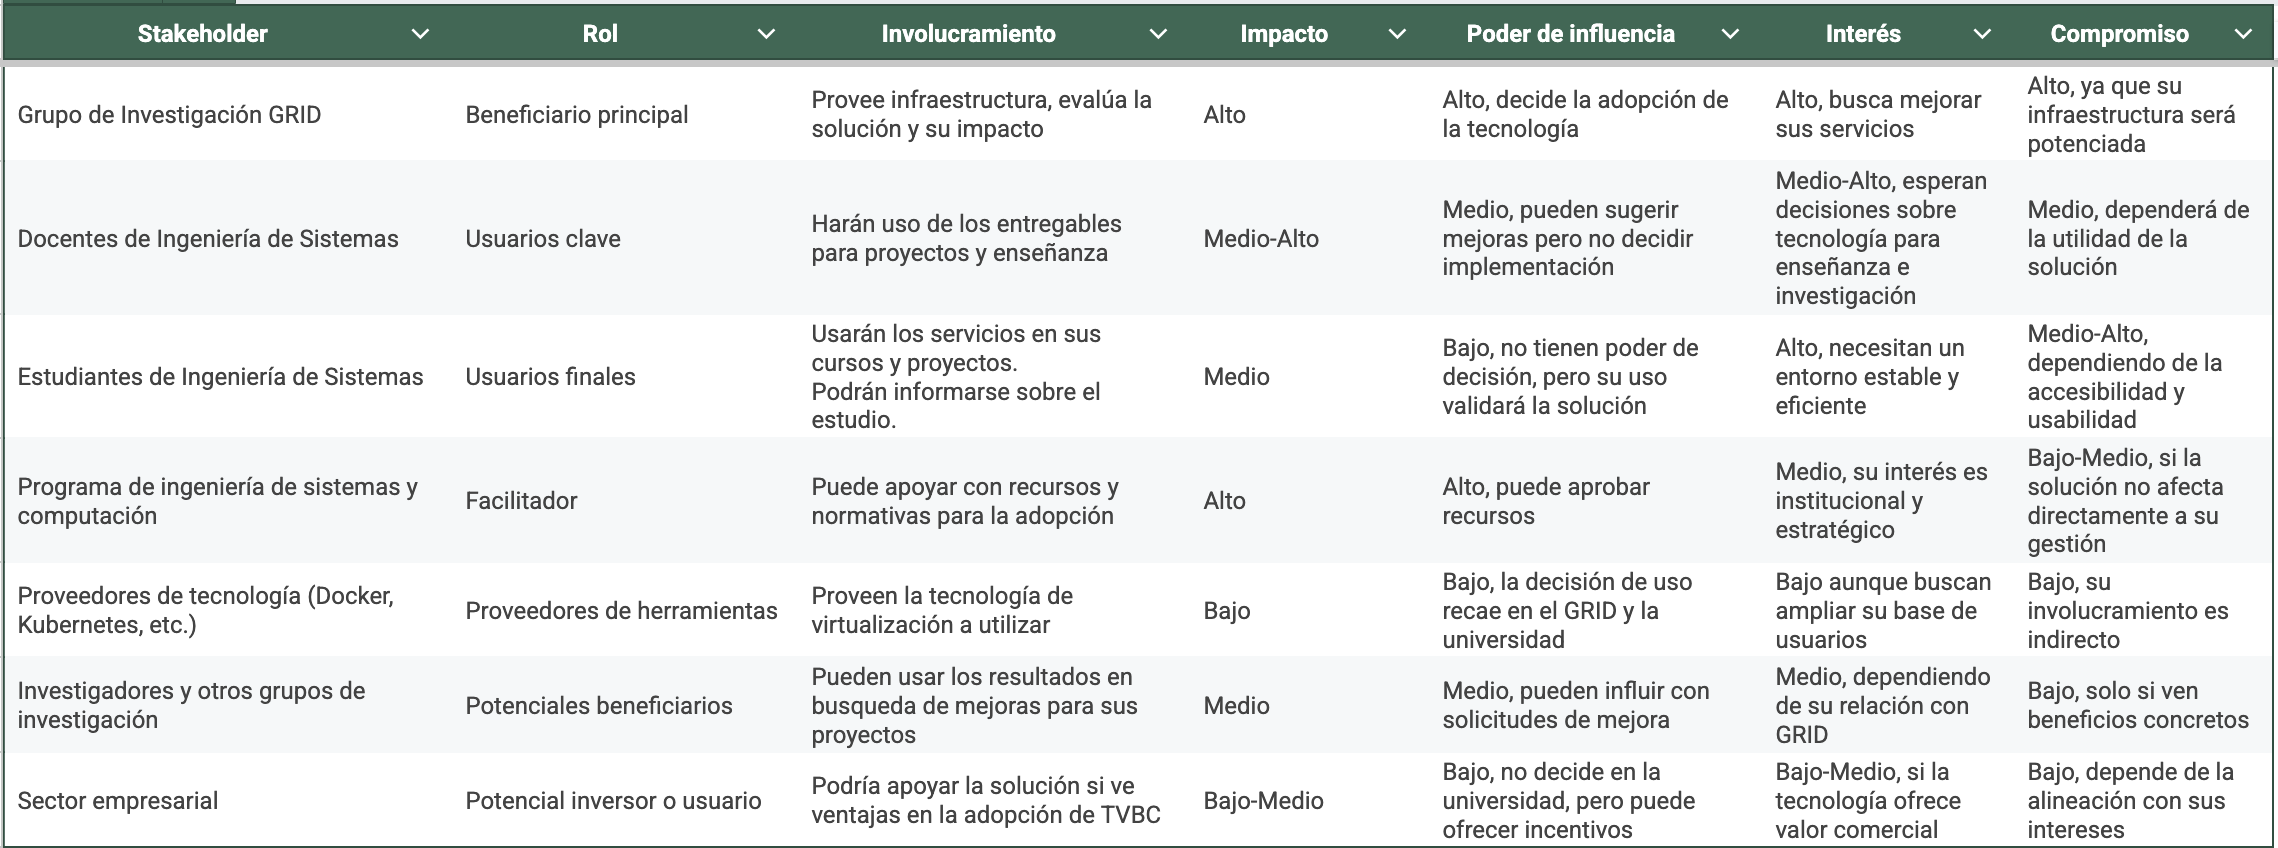
\includegraphics[width=\textwidth]{tablas-images/cp1/definicionStakeholders.png}
    \caption{Análisis de stakeholders del proyecto}
    \label{tab:tabla-stakeholders}
\end{table}

\section{Priorización de stakeholders}
Tras la identificación de los \textit{stakeholders}, se realizó un proceso de priorización para determinar cuáles poseen mayor impacto y poder de decisión en el proyecto. Esta clasificación resulta crucial para establecer estrategias de comunicación, gestión de expectativas y participación activa en la definición de requerimientos. De esta manera, se garantiza que los actores más influyentes en la toma de decisiones y en la adopción tecnológica sean atendidos de forma prioritaria, aumentando las probabilidades de éxito en la implementación.  

\begin{figure}[H]
    \centering
    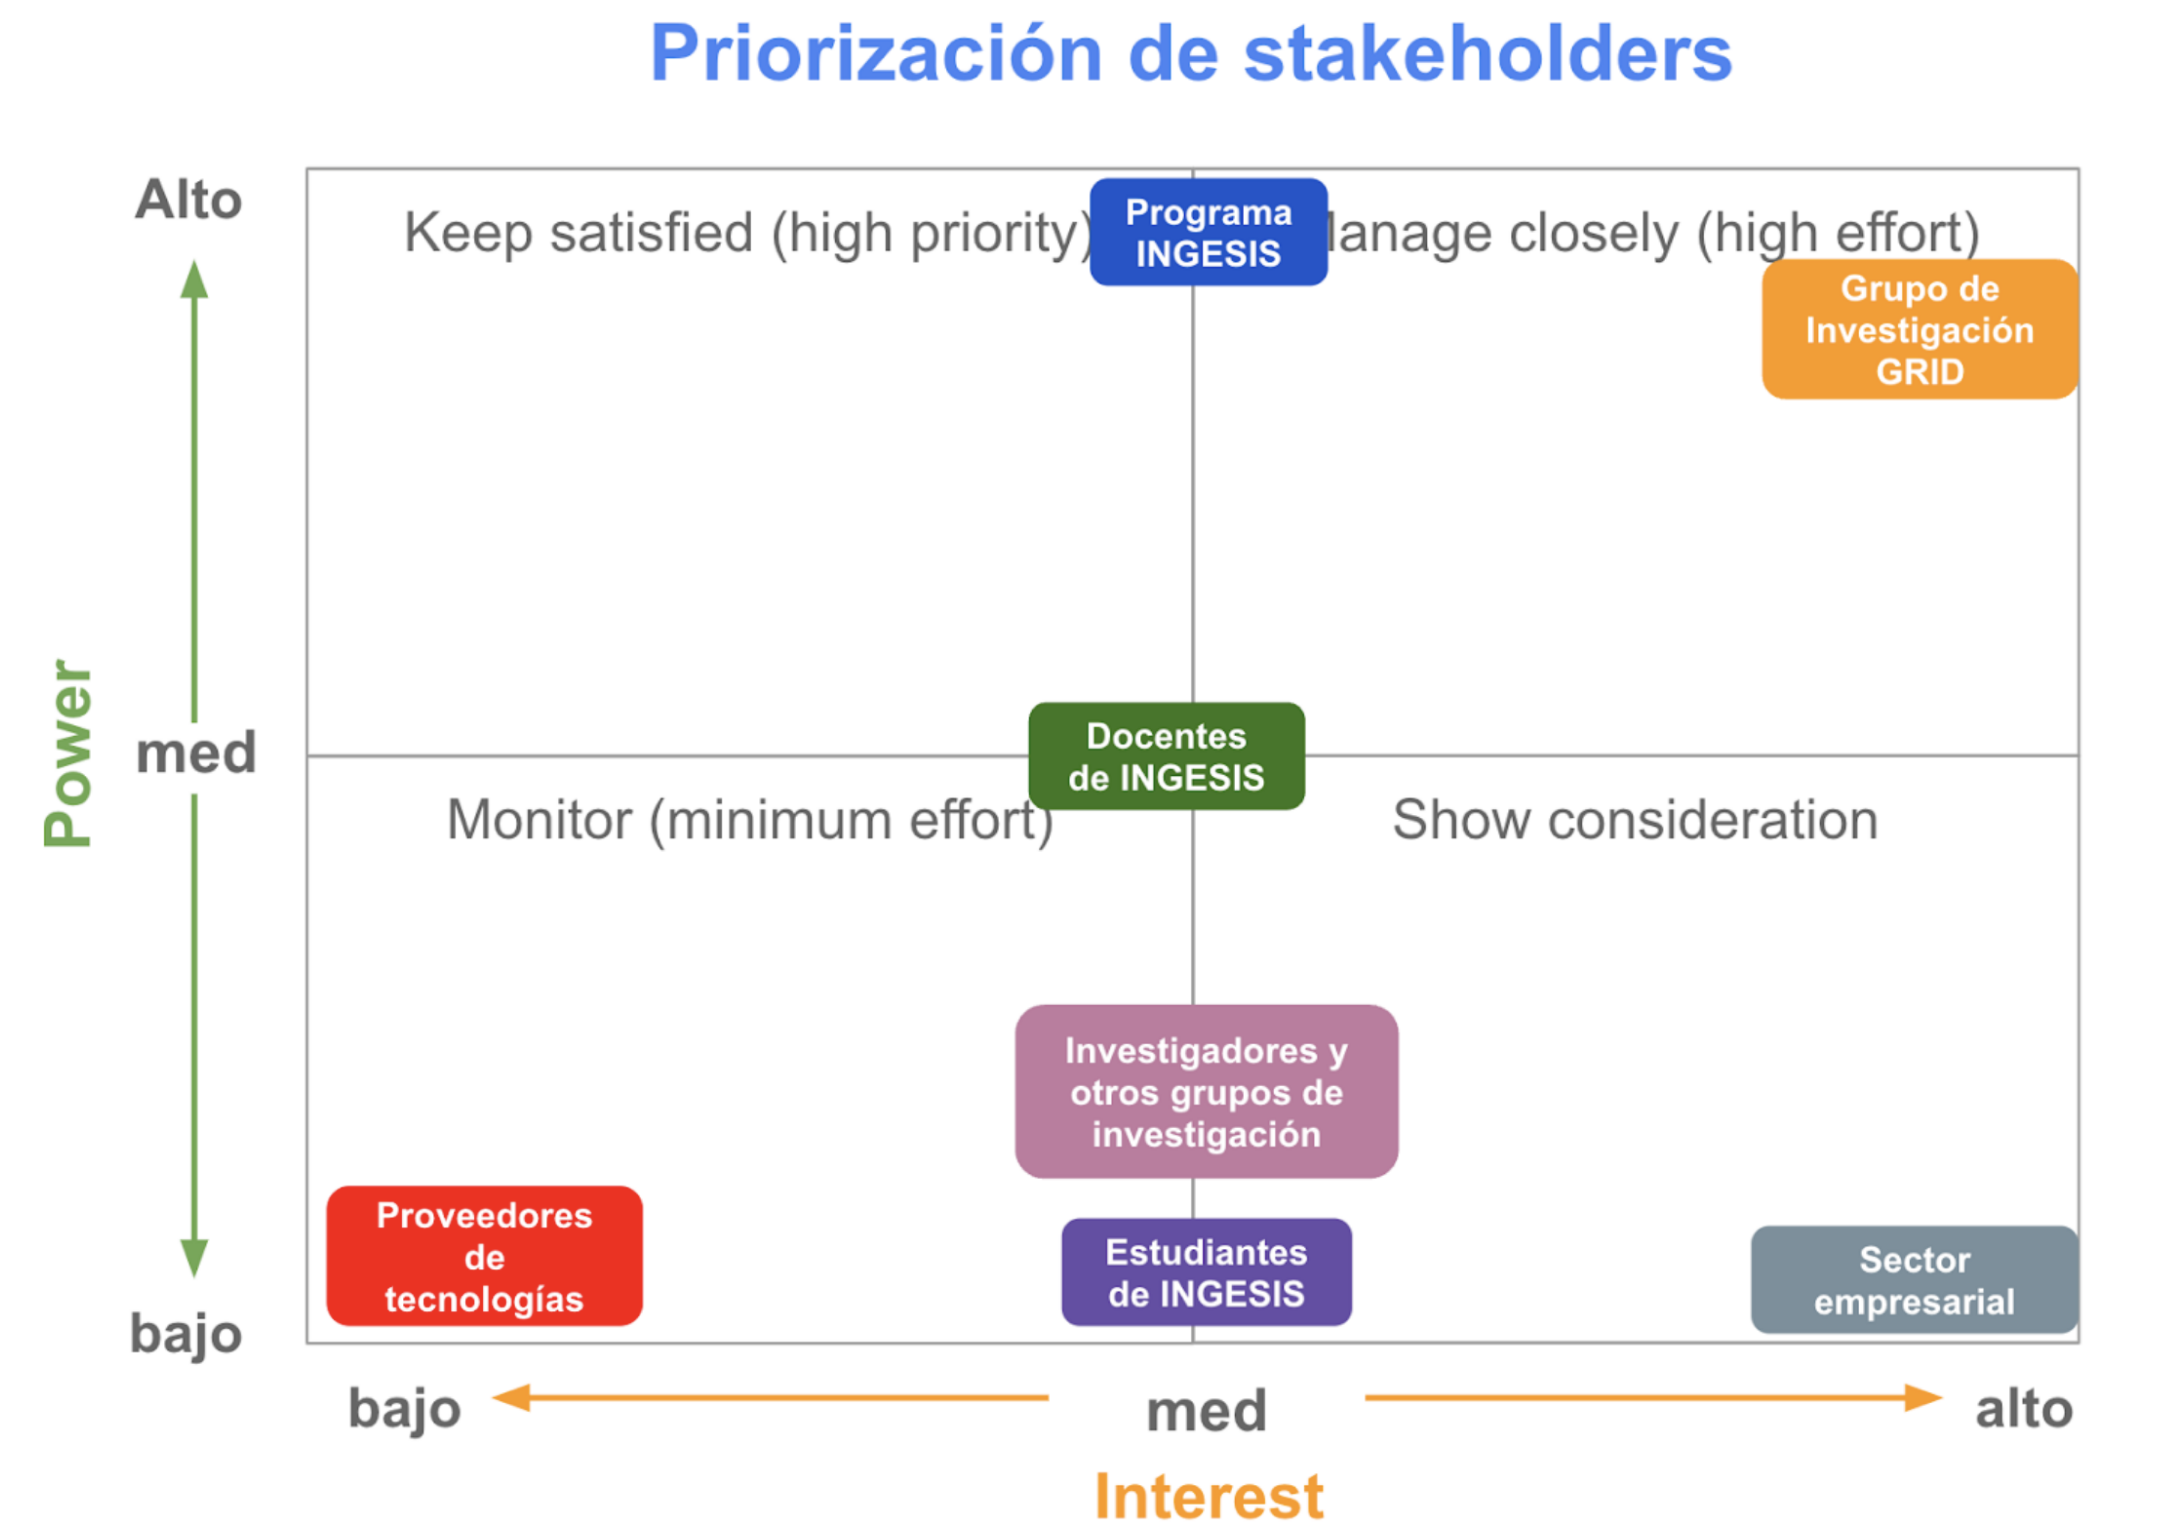
\includegraphics[width=\textwidth] {tablas-images/cp1/priorizacionStakeholders.png}
    \caption{Priorización de stakeholders del proyecto}\label{fig:tabla-priorizacion-stakeholders}
\end{figure}

\section{Integrantes y áreas de trabajo del GRID}
El \GRID está conformado por un equipo multidisciplinario de investigadores y profesionales que, desde sus diferentes áreas de experticia, contribuyen al avance en campos como computación de alto rendimiento, \textit{big data}, inteligencia artificial, redes y desarrollo de software. A continuación, se listan sus integrantes junto con las principales líneas de investigación y trabajo:  

\begin{itemize}
  \item \href{https://scienti.minciencias.gov.co/cvlac/visualizador/generarCurriculoCv.do?cod_rh=0000210897}{\underline{{\textbf{Christian Andrés Candela Uribe}}}}: Microservicios, desarrollo de software, minería de datos, infraestructura TI.\@
  \item \href{https://scienti.minciencias.gov.co/cvlac/visualizador/generarCurriculoCv.do?cod_rh=0001383939}{\underline{{\textbf{Luis Eduardo Sepúlveda Rodríguez}}}}: Infraestructura de TI, HPC, computación paralela.
  \item \href{https://scienti.minciencias.gov.co/cvlac/visualizador/generarCurriculoCv.do?cod_rh=0001638854}{\underline{{\textbf{Carlos Andrés Flórez Villarraga}}}}: Programación y algoritmia, inteligencia artificial.
  \item \href{https://scienti.minciencias.gov.co/cvlac/visualizador/generarCurriculoCv.do?cod_rh=0001343801}{\underline{{\textbf{Carlos Eduardo Gómez Montoya}}}}: Redes, ingeniería de software, cloud computing.
  \item \href{https://scienti.minciencias.gov.co/cvlac/visualizador/generarCurriculoCv.do?cod_rh=0001398775}{\underline{{\textbf{Sergio Augusto Cardona Torres}}}}: Big data y análisis de datos, ingeniería de software, sistemas adaptativos, informática educativa.
  \item \href{https://scienti.minciencias.gov.co/cvlac/visualizador/generarCurriculoCv.do?cod_rh=0000193550}{\underline{{\textbf{Sonia Jaramillo Valbuena}}}}: Big data, electroquímica, inteligencia artificial.
  \item \href{https://scienti.minciencias.gov.co/cvlac/visualizador/generarCurriculoCv.do?cod_rh=0000283495}{\underline{{\textbf{Julián Esteban Gutiérrez Posada}}}}: Microservicios, desarrollo de software, minería de datos, infraestructura TI, HPC, computación paralela, redes, ingeniería de software.
\end{itemize}

La diversidad de líneas de trabajo de los integrantes fortalece la capacidad del grupo para abordar proyectos de carácter transversal y multidisciplinario, lo cual resulta particularmente relevante para el diseño e implementación de soluciones arquitectónicas soportadas en tecnologías de virtualización.

\section{Misión del GRID}
La misión del GRID es heredada de la Universidad del Quindío. A continuación se presenta la misión del GRID:\@

\begin{quote}
\textit{La Universidad del Quindío contribuye a la transformación de la sociedad, mediante la formación integral desde el ser, el saber y el hacer, de líderes reflexivos y gestores del cambio; con estándares de calidad, a través de una oferta de formación en diferentes metodologías, que responda a una sociedad basada en el conocimiento; una investigación pertinente, que aporte a la solución de las problemáticas del desarrollo e integrada con la extensión y proyección social; educando en tiempos del posconflicto y de la consolidación de la paz, apoyada en una gestión creativa y con estándares de calidad.}
\end{quote}

A partir de esta misión, se identifican los siguientes pilares fundamentales:

\begin{itemize}
    \item \textbf{Docencia:} La Universidad del Quindío contribuye a la transformación de la sociedad, mediante la formación integral desde el ser, el saber y el hacer, de líderes reflexivos y gestores del cambio; con estándares de calidad, a través de una oferta de formación en diferentes metodologías, que responda a una sociedad basada en el conocimiento.

    \item \textbf{Investigación:} Una investigación pertinente, que aporte a la solución de las problemáticas del desarrollo e integrada con la extensión y proyección social.

    \item \textbf{Extensión y Desarrollo Social:} Apoyada en una gestión creativa y con estándares de calidad.

    \item \textbf{Responsabilidad Social:} Educando en tiempos del posconflicto y de la consolidación de la paz.
\end{itemize}

\section{Visión del GRID}
La misión de la Universidad del Quindío se complementa con su visión institucional, la cual también es adoptada por el \GRID. A continuación se presenta la visión del \GRID:\@

\begin{quote}
\textit{En el año 2025, la Universidad del Quindío estará consolidada como una institución \textit{Pertinente --- Creativa --- Integradora}, acreditada de alta calidad, con reconocimiento nacional e internacional en sus procesos de formación a través de diferentes metodologías, de investigación, extensión, proyección y responsabilidad social.}
\end{quote}

A partir de esta visión, se destacan los siguientes enfoques estratégicos:

\begin{itemize}
    \item \textbf{Gestión:} La Universidad del Quindío estará consolidada como una institución \textit{Pertinente --- Creativa --- Integradora}.

    \item \textbf{Docencia:} Acreditada de alta calidad en sus procesos de formación a través de diferentes metodologías.

    \item \textbf{Investigación:} Consolidada como pertinente y de alta calidad en sus procesos de investigación.

    \item \textbf{Extensión y Desarrollo Social:} Procesos creativos e integradores en proyección social.

    \item \textbf{Responsabilidad Social:} Reconocimientos en sus procesos de responsabilidad social.
\end{itemize}

\section{Impacto del proyecto en el GRID}

El proyecto tiene como objetivo apoyar los procesos de docencia, investigación
y extensión mediante la especificación de una arquitectura de tecnologías de 
virtualización basada en contenedores (\VBC). 

Este trabajo se enfoca en la identificación de una tecnología de contenerización que 
\textbf{agregue valor a los procesos del \GRID}, beneficiando a docentes, estudiantes
y cualquier parte interesada que participe en los proyectos y actividades desarrolladas 
por este grupo de investigación.

\section{Caracterización de la infraestructura tecnológica del GRID}
En el siguiente formato se van a especificar las características técnicas de la infraestructura tecnológica del GRID disponible para temas de virtualización.\ \href{https://docs.google.com/spreadsheets/d/14NBv72ucVTrLqGIldYdIsjdBGt3QlgwcblcVRis-DaQ/edit?usp=sharing}{Macro de la ficha técnica}
% Archivo de caracterización de infraestructura corregido

% Torre HP 1
\begin{table}[H]
\centering
\caption{Ficha técnica --- Torre 1}\label{tab:torre-hp-1}
\begin{tabular}{|p{0.6\textwidth}|p{0.3\textwidth}|}
\hline
\multicolumn{2}{|l|}{\textbf{DESCRIPCIÓN FÍSICA:} Servidor tipo torre} \\ \hline
\textbf{TIPO DE RECURSO:} Torre &
\multirow{5}{*}{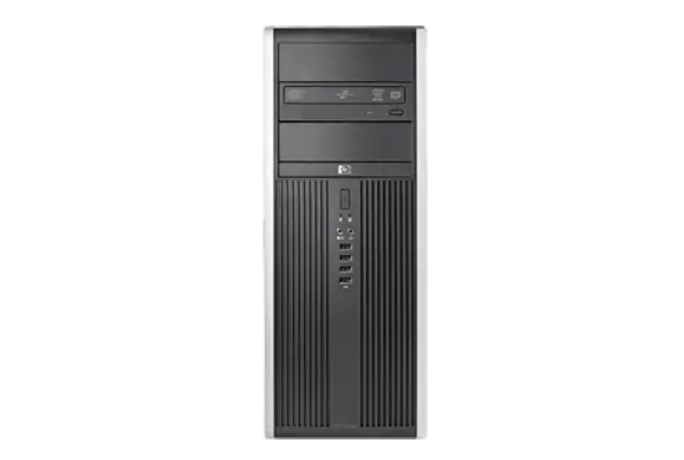
\includegraphics[width=0.25\textwidth,height=4cm,keepaspectratio]{tablas-images/cp1/torres/torre-1.png}} \\ \cline{1-1}
\textbf{MODELO:} Desconocido & \\ \cline{1-1}
\textbf{MARCA:} HP & \\ \cline{1-1}
\textbf{CÓDIGO DE INVENTARIO:} 7 24390 49867 3 & \\ \cline{1-1}
\textbf{NÚMERO EN CPD:} 14 & \\ \hline
\multicolumn{2}{|l|}{\textbf{ESPECIFICACIONES TÉCNICAS}} \\ \hline
\multicolumn{2}{|p{0.95\textwidth}|}{
\footnotesize
- 8 entradas USB (4 al frente, 4 en la parte trasera)
- Entrada de audio y microfono
- Entrada HDMI
- Lector de DVDs
- 3 puertos Ethernet (Parte trasera)
- Entrada Displayport
- Puertos PS/2 (Teclado y Ratón)
} \\ \hline
\multicolumn{2}{|l|}{\textbf{PROPÓSITO:} Hipervisor de XCP-ng} \\ \hline
\multicolumn{2}{|l|}{\textbf{OPORTUNIDAD DE USO:} Proyectos del \GRID} \\ \hline
\multicolumn{2}{|p{0.9\textwidth}|}{\textbf{OBSERVACIONES:} El Equipo no tiene modelo. El equipo está diseñado para usuario final pero fue adaptado para entornos de virtualización.} \\ \hline
\end{tabular}
\end{table}


% Torre 2
\begin{table}[H]
\centering
\caption{Ficha técnica --- Torre 2}\label{tab:torre-2}
\begin{tabular}{|p{0.6\textwidth}|p{0.3\textwidth}|}
\hline
\multicolumn{2}{|l|}{\textbf{DESCRIPCIÓN FÍSICA:} Servidor tipo torre} \\ \hline
\textbf{TIPO DE RECURSO:} Torre & 
\multirow{5}{*}{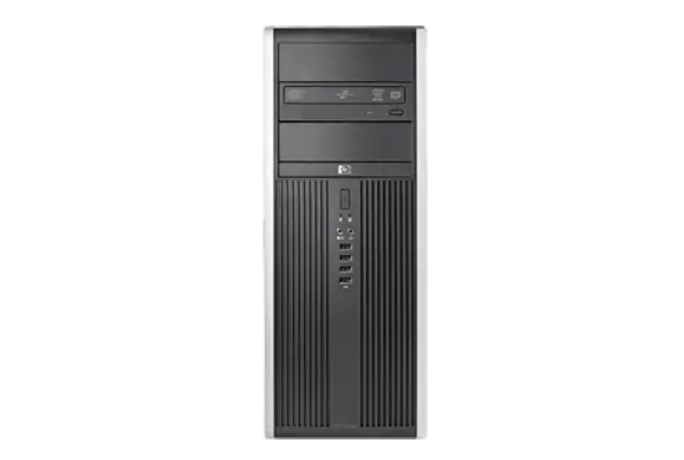
\includegraphics[width=0.25\textwidth,height=4cm,keepaspectratio]{tablas-images/cp1/torres/torre-1.png}} \\ \cline{1-1}
\textbf{MODELO:} Desconocido & \\ \cline{1-1}
\textbf{MARCA:} HP & \\ \cline{1-1}
\textbf{CÓDIGO DE INVENTARIO:} 7 24390 49861 1 & \\ \cline{1-1}
\textbf{NÚMERO EN CPD:} 12 & \\ \hline
\multicolumn{2}{|l|}{\textbf{ESPECIFICACIONES TÉCNICAS}} \\ \hline
\multicolumn{2}{|p{0.95\textwidth}|}{
\footnotesize
- 8 entradas USB (4 al frente, 4 en la parte trasera)
- Entrada de audio y microfono
- Entrada HDMI
- Lector de DVDs
- 3 puertos Ethernet (Parte trasera)
- Entrada Displayport
- Puertos PS/2 (Teclado y Ratón)
} \\ \hline
\multicolumn{2}{|l|}{\textbf{PROPÓSITO:} Hipervisor de XCP-ng} \\ \hline
\multicolumn{2}{|l|}{\textbf{OPORTUNIDAD DE USO:} Proyectos del \GRID} \\ \hline
\multicolumn{2}{|p{0.9\textwidth}|}{\textbf{OBSERVACIONES:} El Equipo no tiene modelo. El equipo está diseñado para usuario final pero fue adaptado para entornos de virtualización.} \\ \hline
\end{tabular}
\end{table}

% Torre 3
\begin{table}[H]
\centering
\caption{Ficha técnica -- Torre 3}
\label{tab:torre-3}
\begin{tabular}{|p{0.6\textwidth}|p{0.3\textwidth}|}
\hline
\multicolumn{2}{|l|}{\textbf{DESCRIPCIÓN FÍSICA:} Servidor tipo torre} \\ \hline
\textbf{TIPO DE RECURSO:} Torre & 
\multirow{5}{*}{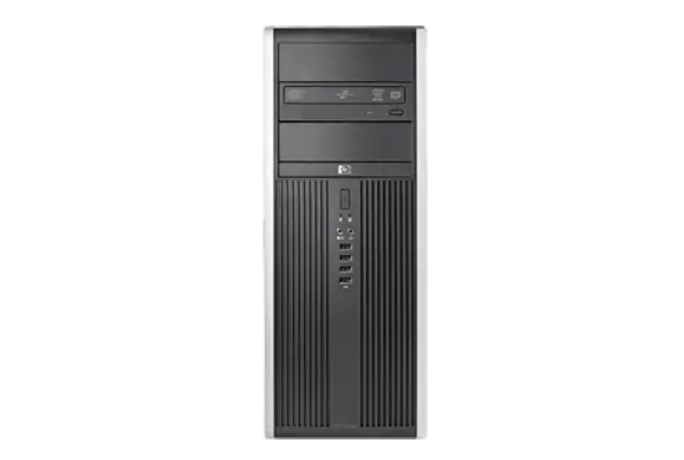
\includegraphics[width=0.25\textwidth,height=4cm,keepaspectratio]{tablas-images/cp1/torres/torre-1.png}} \\ \cline{1-1}
\textbf{MODELO:} Desconocido & \\ \cline{1-1}
\textbf{MARCA:} HP & \\ \cline{1-1}
\textbf{CÓDIGO DE INVENTARIO:} 7 24390 49969 4 & \\ \cline{1-1}
\textbf{NÚMERO EN CPD:} 13 & \\ \hline
\multicolumn{2}{|l|}{\textbf{ESPECIFICACIONES TÉCNICAS}} \\ \hline
\multicolumn{2}{|p{0.95\textwidth}|}{
\footnotesize
- 8 entradas USB (4 al frente, 4 en la parte trasera)
- Entrada de audio y microfono
- Entrada HDMI
- Lector de DVDs
- 3 puertos Ethernet (Parte trasera)
- Entrada Displayport
- Puertos PS/2 (Teclado y Ratón)
} \\ \hline
\multicolumn{2}{|l|}{\textbf{PROPÓSITO:} Hipervisor de XCP-ng} \\ \hline
\multicolumn{2}{|l|}{\textbf{OPORTUNIDAD DE USO:} Proyectos del \GRID} \\ \hline
\multicolumn{2}{|p{0.9\textwidth}|}{\textbf{OBSERVACIONES:} El Equipo no tiene modelo. El equipo está diseñado para usuario final pero fue adaptado para entornos de virtualización.} \\ \hline
\end{tabular}
\end{table}

% Torre 4
\begin{table}[H]
\centering
\caption{Ficha técnica --- Torre 4}
\label{tab:torre-4}
\begin{tabular}{|p{0.6\textwidth}|p{0.3\textwidth}|}
\hline
\multicolumn{2}{|l|}{\textbf{DESCRIPCIÓN FÍSICA:} Servidor tipo torre} \\ \hline
\textbf{TIPO DE RECURSO:} Torre & 
\multirow{5}{*}{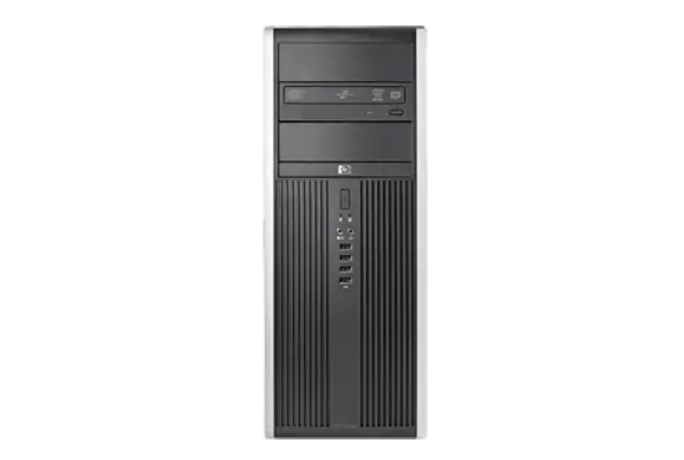
\includegraphics[width=0.25\textwidth,height=4cm,keepaspectratio]{tablas-images/cp1/torres/torre-1.png}} \\ \cline{1-1}
\textbf{MODELO:} Desconocido & \\ \cline{1-1}
\textbf{MARCA:} HP & \\ \cline{1-1}
\textbf{CÓDIGO DE INVENTARIO:} 7 24390 49879 4 & \\ \cline{1-1}
\textbf{NÚMERO EN CPD:} 14 & \\ \hline
\multicolumn{2}{|l|}{\textbf{ESPECIFICACIONES TÉCNICAS}} \\ \hline
\multicolumn{2}{|p{0.95\textwidth}|}{
\footnotesize
- 8 entradas USB (4 al frente, 4 en la parte trasera)
- Entrada de audio y microfono
- Entrada HDMI
- Lector de DVDs
- 3 puertos Ethernet (Parte trasera)
- Entrada Displayport
- Puertos PS/2 (Teclado y Ratón)
} \\ \hline
\multicolumn{2}{|l|}{\textbf{PROPÓSITO:} Hipervisor de XCP-ng} \\ \hline
\multicolumn{2}{|l|}{\textbf{OPORTUNIDAD DE USO:} Proyectos del \GRID} \\ \hline
\multicolumn{2}{|p{0.9\textwidth}|}{\textbf{OBSERVACIONES:} El Equipo no tiene modelo. El equipo está diseñado para usuario final pero fue adaptado para entornos de virtualización.} \\ \hline
\end{tabular}
\end{table}

% Torre 5
\begin{table}[H]
\centering
\caption{Ficha técnica --- Torre 5}
\label{tab:torre-5}
\begin{tabular}{|p{0.6\textwidth}|p{0.3\textwidth}|}
\hline
\multicolumn{2}{|l|}{\textbf{DESCRIPCIÓN FÍSICA:} Servidor tipo torre} \\ \hline
\textbf{TIPO DE RECURSO:} Torre & 
\multirow{5}{*}{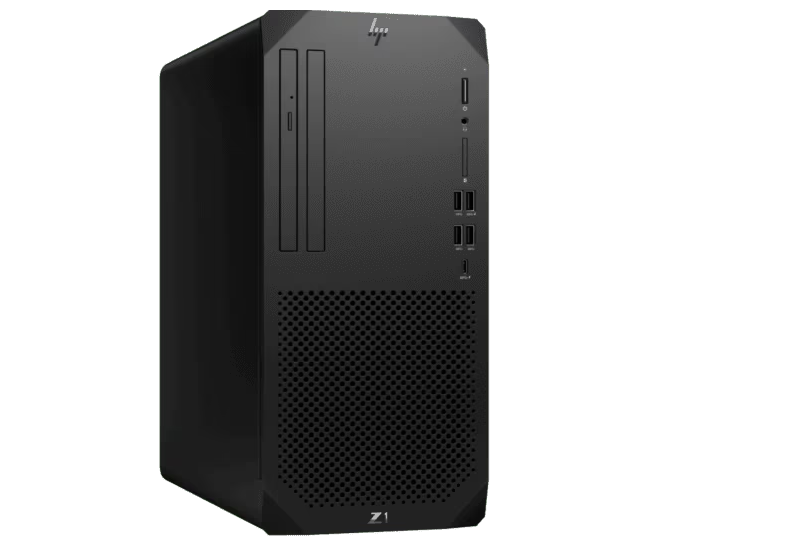
\includegraphics[width=0.25\textwidth,height=4cm,keepaspectratio]{tablas-images/cp1/torres/torre-2.png}} \\ \cline{1-1}
\textbf{MODELO:} G9 & \\ \cline{1-1}
\textbf{MARCA:} HP & \\ \cline{1-1}
\textbf{CÓDIGO DE INVENTARIO:} 72992 & \\ \cline{1-1}
\textbf{NÚMERO EN CPD:} 22 & \\ \hline
\multicolumn{2}{|l|}{\textbf{ESPECIFICACIONES TÉCNICAS}} \\ \hline
\multicolumn{2}{|p{0.95\textwidth}|}{
\footnotesize
- 9 entradas USB (4 al frente, 5 en la parte trasera)
- Entrada de audio y microfono
- Entrada HDMI
- Lector de DVDs
- 1 puerto Ethernet (Parte trasera)
- 2 Entrada Displayport
- Procesador Intel vPro i9
} \\ \hline
\multicolumn{2}{|l|}{\textbf{PROPÓSITO:} Hipervisor de XCP-ng} \\ \hline
\multicolumn{2}{|l|}{\textbf{OPORTUNIDAD DE USO:} Proyectos del \GRID} \\ \hline
\multicolumn{2}{|p{0.9\textwidth}|}{\textbf{OBSERVACIONES:} El equipo está diseñado para usuario final pero fue adaptado para entornos de virtualización.} \\ \hline
\end{tabular}
\end{table}

% Torre 6
\begin{table}[H]
\centering
\caption{Ficha técnica --- Torre 6}
\label{tab:torre-6}
\begin{tabular}{|p{0.6\textwidth}|p{0.3\textwidth}|}
\hline
\multicolumn{2}{|l|}{\textbf{DESCRIPCIÓN FÍSICA:} Servidor tipo torre} \\ \hline
\textbf{TIPO DE RECURSO:} Torre & 
\multirow{5}{*}{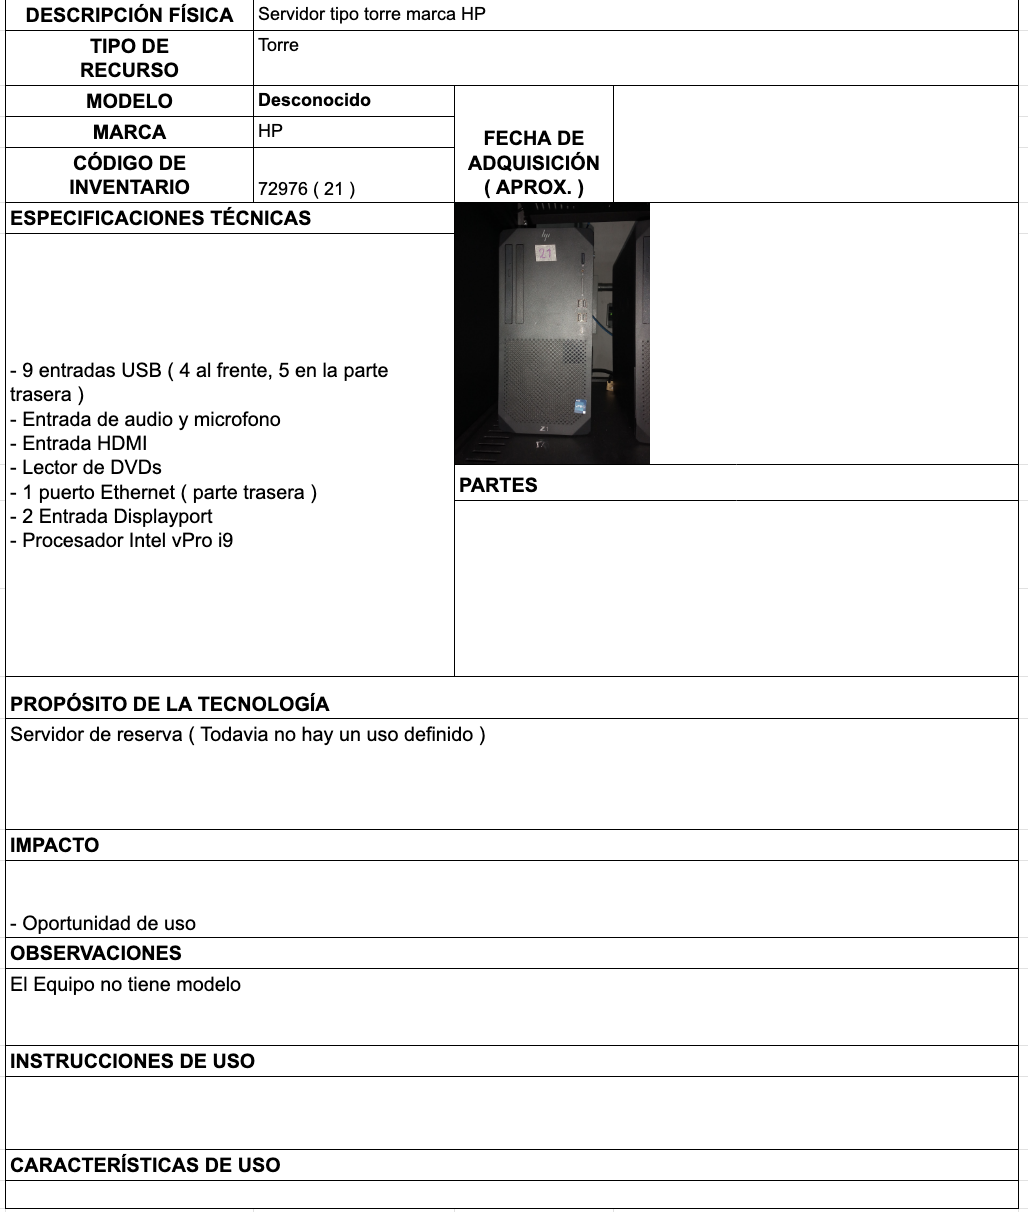
\includegraphics[width=0.25\textwidth,height=4cm,keepaspectratio]{tablas-images/cp1/torres/torre-6.png}} \\ \cline{1-1}
\textbf{MODELO:} Por definir & \\ \cline{1-1}
\textbf{MARCA:} Por definir & \\ \cline{1-1}
\textbf{CÓDIGO DE INVENTARIO:} Por definir & \\ \cline{1-1}
\textbf{FECHA DE ADQUISICIÓN (APROX.):} & \\ \hline
\multicolumn{2}{|l|}{\textbf{ESPECIFICACIONES TÉCNICAS}} \\ \hline
\multicolumn{2}{|p{0.95\textwidth}|}{
\footnotesize
Especificaciones por definir según imagen adjunta
} \\ \hline
\multicolumn{2}{|l|}{\textbf{PROPÓSITO:} Por definir} \\ \hline
\multicolumn{2}{|l|}{\textbf{IMPACTO:} Por evaluar} \\ \hline
\multicolumn{2}{|l|}{\textbf{OBSERVACIONES:} Ver imagen para detalles} \\ \hline
\end{tabular}
\end{table}

% Torre 7
\begin{table}[H]
\centering
\caption{Ficha técnica -- Torre 7}
\label{tab:torre-7}
\begin{tabular}{|p{0.6\textwidth}|p{0.3\textwidth}|}
\hline
\multicolumn{2}{|l|}{\textbf{DESCRIPCIÓN FÍSICA:} Servidor tipo torre} \\ \hline
\textbf{TIPO DE RECURSO:} Torre & 
\multirow{5}{*}{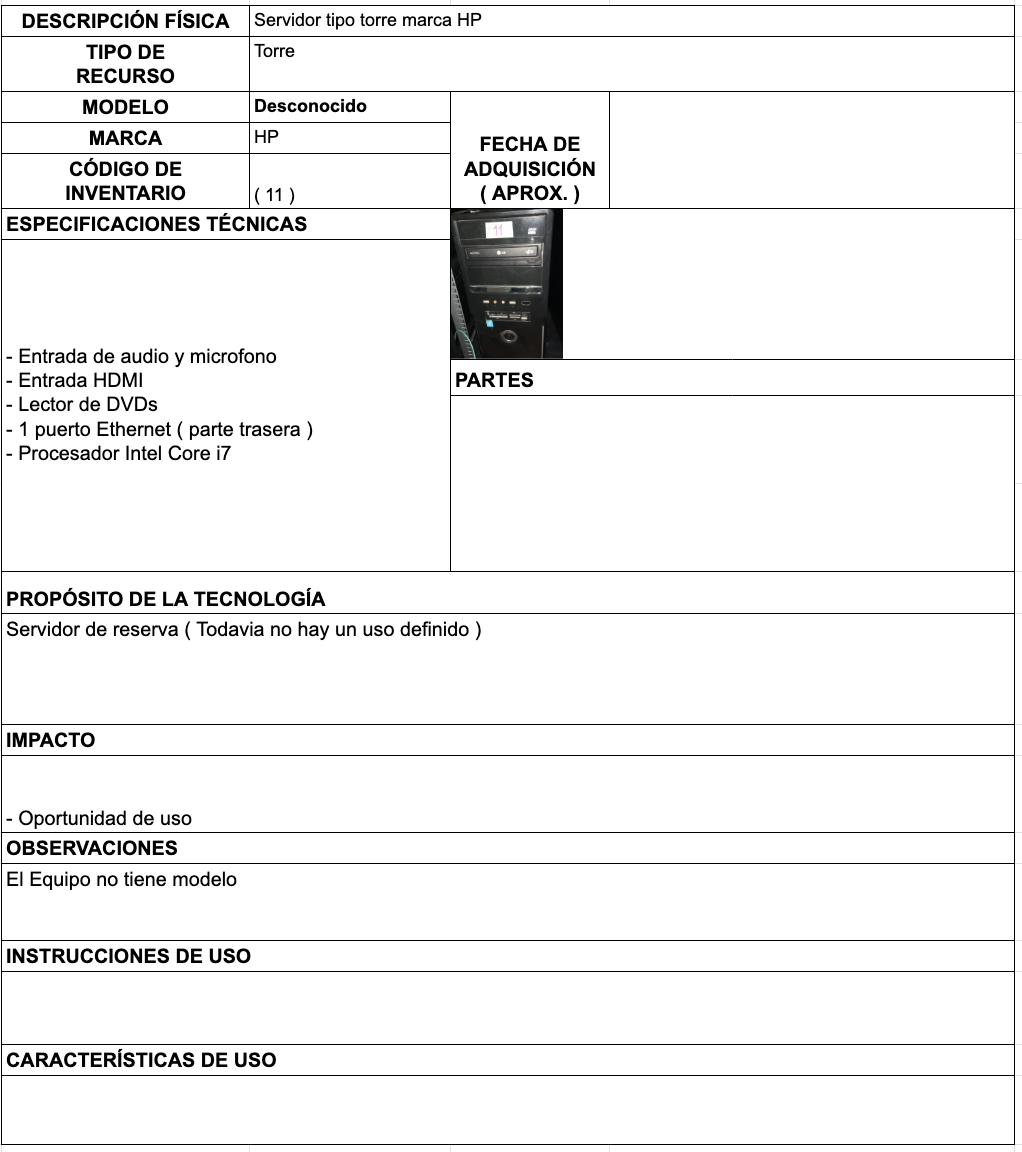
\includegraphics[width=0.25\textwidth,height=4cm,keepaspectratio]{tablas-images/cp1/torres/torre-7.png}} \\ \cline{1-1}
\textbf{MODELO:} Por definir & \\ \cline{1-1}
\textbf{MARCA:} Por definir & \\ \cline{1-1}
\textbf{CÓDIGO DE INVENTARIO:} Por definir & \\ \cline{1-1}
\textbf{FECHA DE ADQUISICIÓN (APROX.):} & \\ \hline
\multicolumn{2}{|l|}{\textbf{ESPECIFICACIONES TÉCNICAS}} \\ \hline
\multicolumn{2}{|p{0.95\textwidth}|}{
\footnotesize
Especificaciones por definir según imagen adjunta
} \\ \hline
\multicolumn{2}{|l|}{\textbf{PROPÓSITO:} Por definir} \\ \hline
\multicolumn{2}{|l|}{\textbf{IMPACTO:} Por evaluar} \\ \hline
\multicolumn{2}{|l|}{\textbf{OBSERVACIONES:} Ver imagen para detalles} \\ \hline
\end{tabular}
\end{table}

% Rack 1
\begin{table}[H]
\centering
\caption{Ficha técnica -- Rack 1}
\label{tab:rack-1}
\begin{tabular}{|p{0.6\textwidth}|p{0.3\textwidth}|}
\hline
\multicolumn{2}{|l|}{\textbf{DESCRIPCIÓN FÍSICA:} Servidor tipo rack} \\ \hline
\textbf{TIPO DE RECURSO:} Rack & 
\multirow{5}{*}{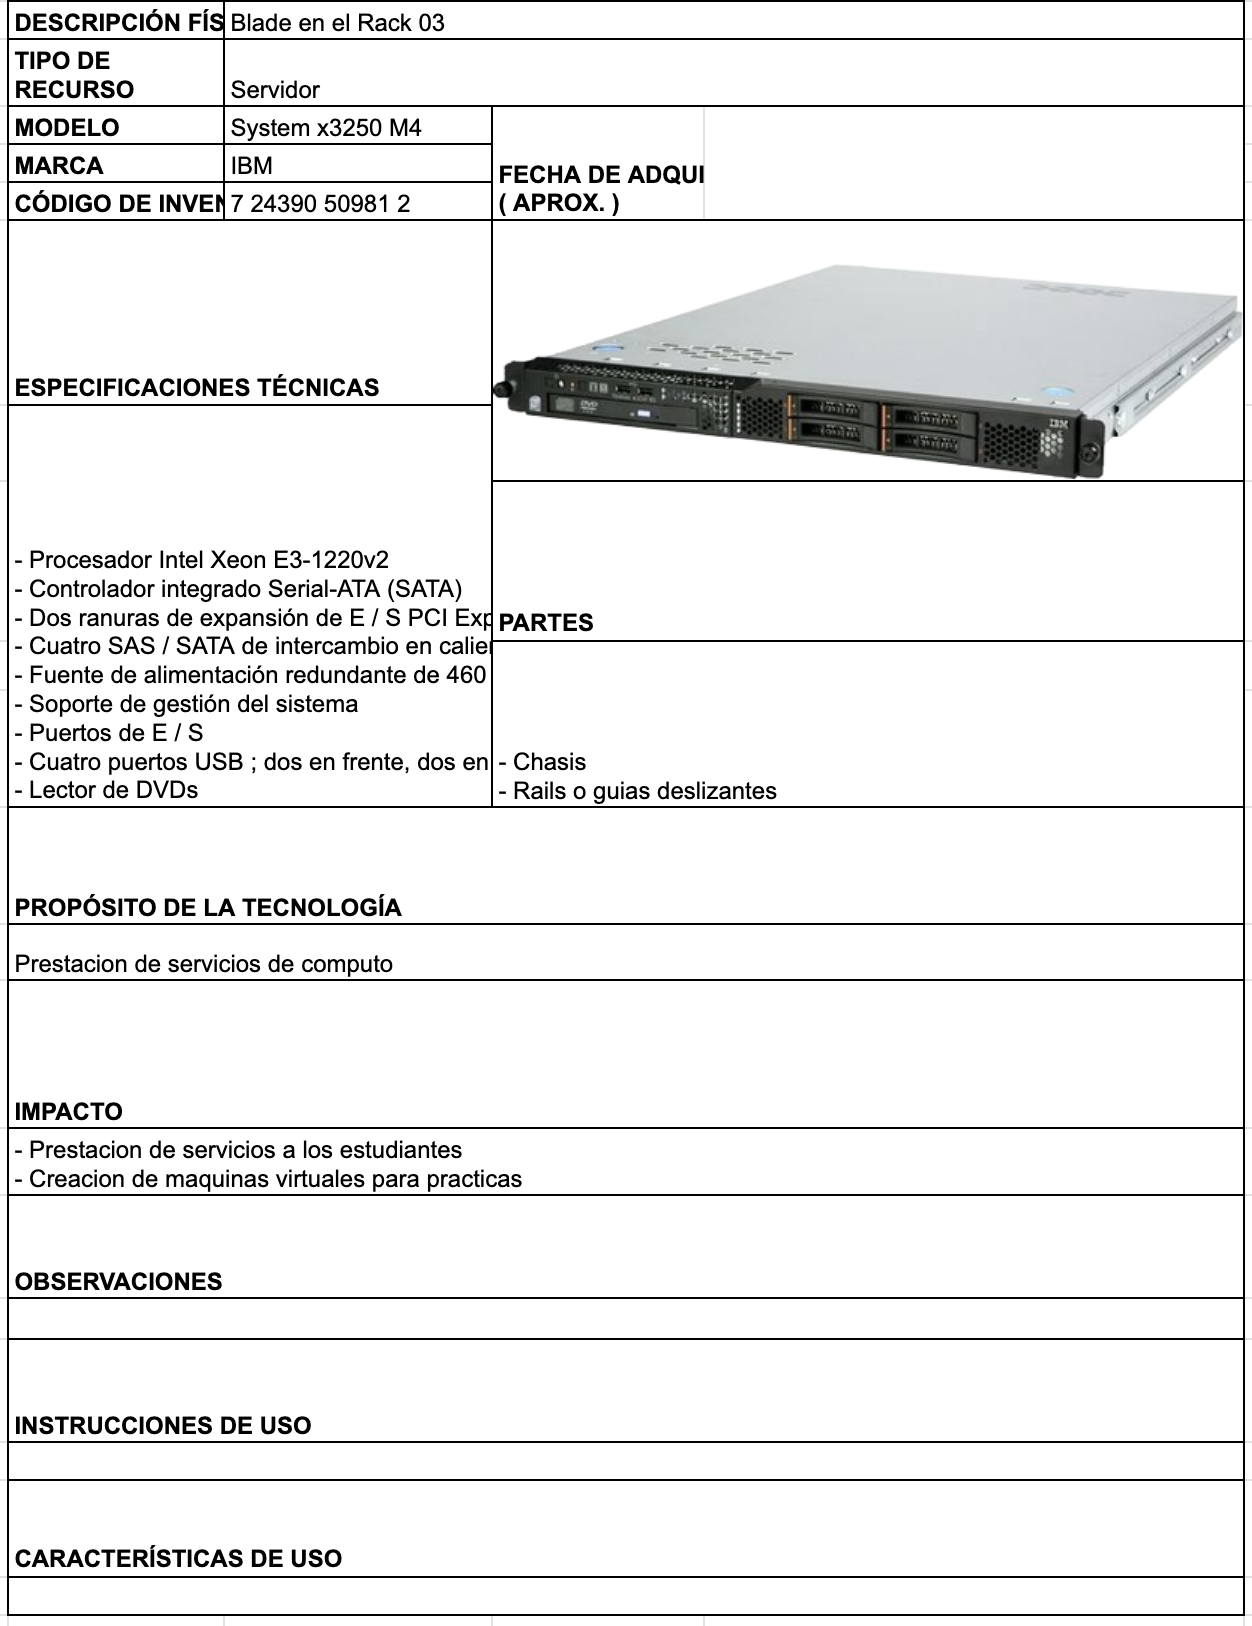
\includegraphics[width=0.25\textwidth,height=4cm,keepaspectratio]{tablas-images/cp1/racks/rack-1.png}} \\ \cline{1-1}
\textbf{MODELO:} Por definir & \\ \cline{1-1}
\textbf{MARCA:} Por definir & \\ \cline{1-1}
\textbf{CÓDIGO DE INVENTARIO:} Por definir & \\ \cline{1-1}
\textbf{FECHA DE ADQUISICIÓN (APROX.):} & \\ \hline
\multicolumn{2}{|l|}{\textbf{ESPECIFICACIONES TÉCNICAS}} \\ \hline
\multicolumn{2}{|p{0.95\textwidth}|}{
\footnotesize
Especificaciones por definir según imagen adjunta
} \\ \hline
\multicolumn{2}{|l|}{\textbf{PROPÓSITO:} Por definir} \\ \hline
\multicolumn{2}{|l|}{\textbf{IMPACTO:} Por evaluar} \\ \hline
\multicolumn{2}{|l|}{\textbf{OBSERVACIONES:} Ver imagen para detalles} \\ \hline
\end{tabular}
\end{table}

% Rack 2
\begin{table}[H]
\centering
\caption{Ficha técnica -- Rack 2}
\label{tab:rack-2}
\begin{tabular}{|p{0.6\textwidth}|p{0.3\textwidth}|}
\hline
\multicolumn{2}{|l|}{\textbf{DESCRIPCIÓN FÍSICA:} Servidor tipo rack} \\ \hline
\textbf{TIPO DE RECURSO:} Rack & 
\multirow{5}{*}{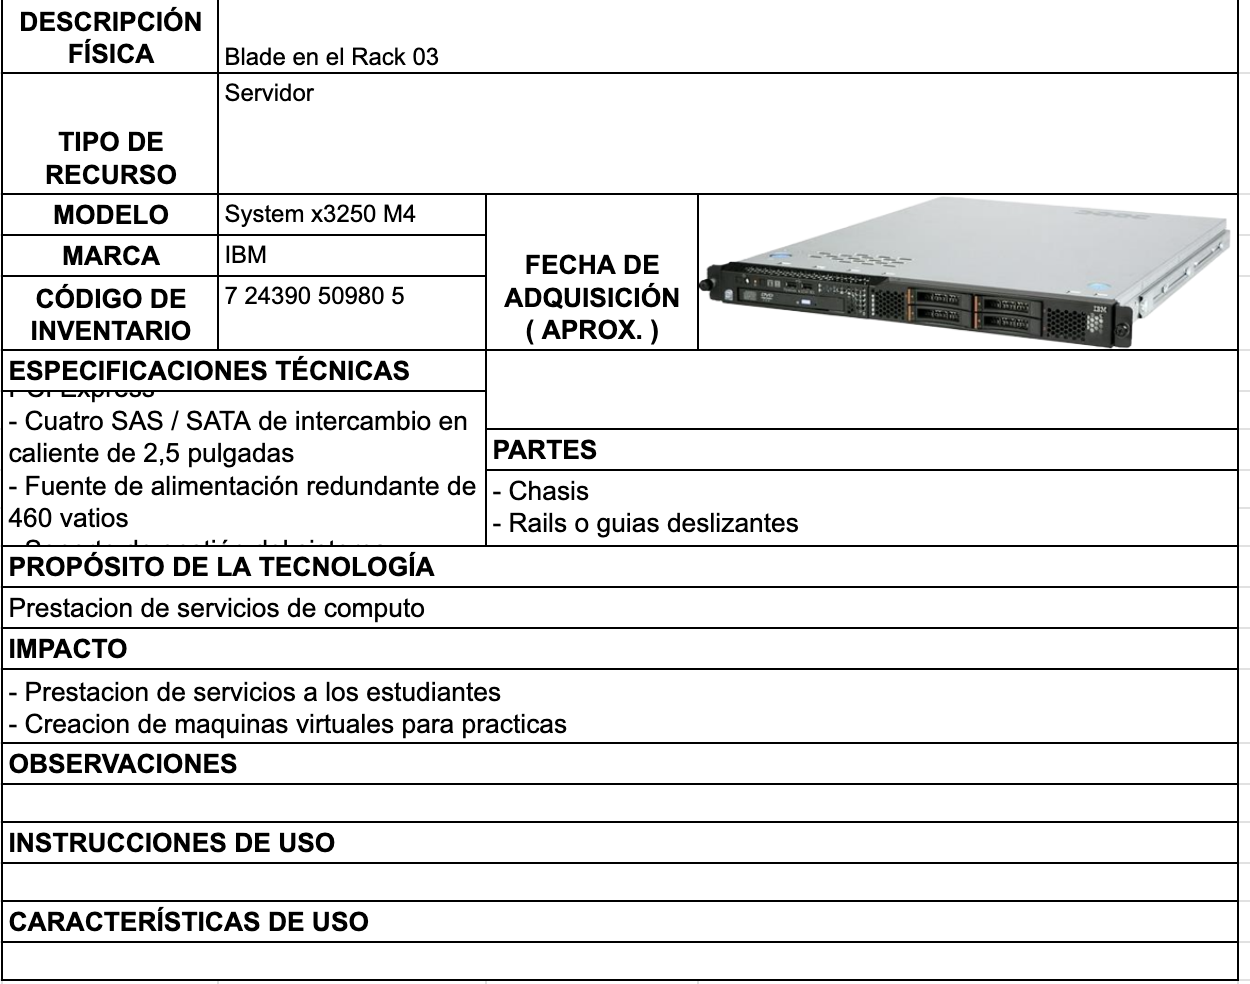
\includegraphics[width=0.25\textwidth,height=4cm,keepaspectratio]{tablas-images/cp1/racks/rack-2.png}} \\ \cline{1-1}
\textbf{MODELO:} Por definir & \\ \cline{1-1}
\textbf{MARCA:} Por definir & \\ \cline{1-1}
\textbf{CÓDIGO DE INVENTARIO:} Por definir & \\ \cline{1-1}
\textbf{FECHA DE ADQUISICIÓN (APROX.):} & \\ \hline
\multicolumn{2}{|l|}{\textbf{ESPECIFICACIONES TÉCNICAS}} \\ \hline
\multicolumn{2}{|p{0.95\textwidth}|}{
\footnotesize
Especificaciones por definir según imagen adjunta
} \\ \hline
\multicolumn{2}{|l|}{\textbf{PROPÓSITO:} Por definir} \\ \hline
\multicolumn{2}{|l|}{\textbf{IMPACTO:} Por evaluar} \\ \hline
\multicolumn{2}{|l|}{\textbf{OBSERVACIONES:} Ver imagen para detalles} \\ \hline
\end{tabular}
\end{table}

% Rack 3
\begin{table}[H]
\centering
\caption{Ficha técnica -- Rack 3}
\label{tab:rack-3}
\begin{tabular}{|p{0.6\textwidth}|p{0.3\textwidth}|}
\hline
\multicolumn{2}{|l|}{\textbf{DESCRIPCIÓN FÍSICA:} Servidor tipo rack} \\ \hline
\textbf{TIPO DE RECURSO:} Rack & 
\multirow{5}{*}{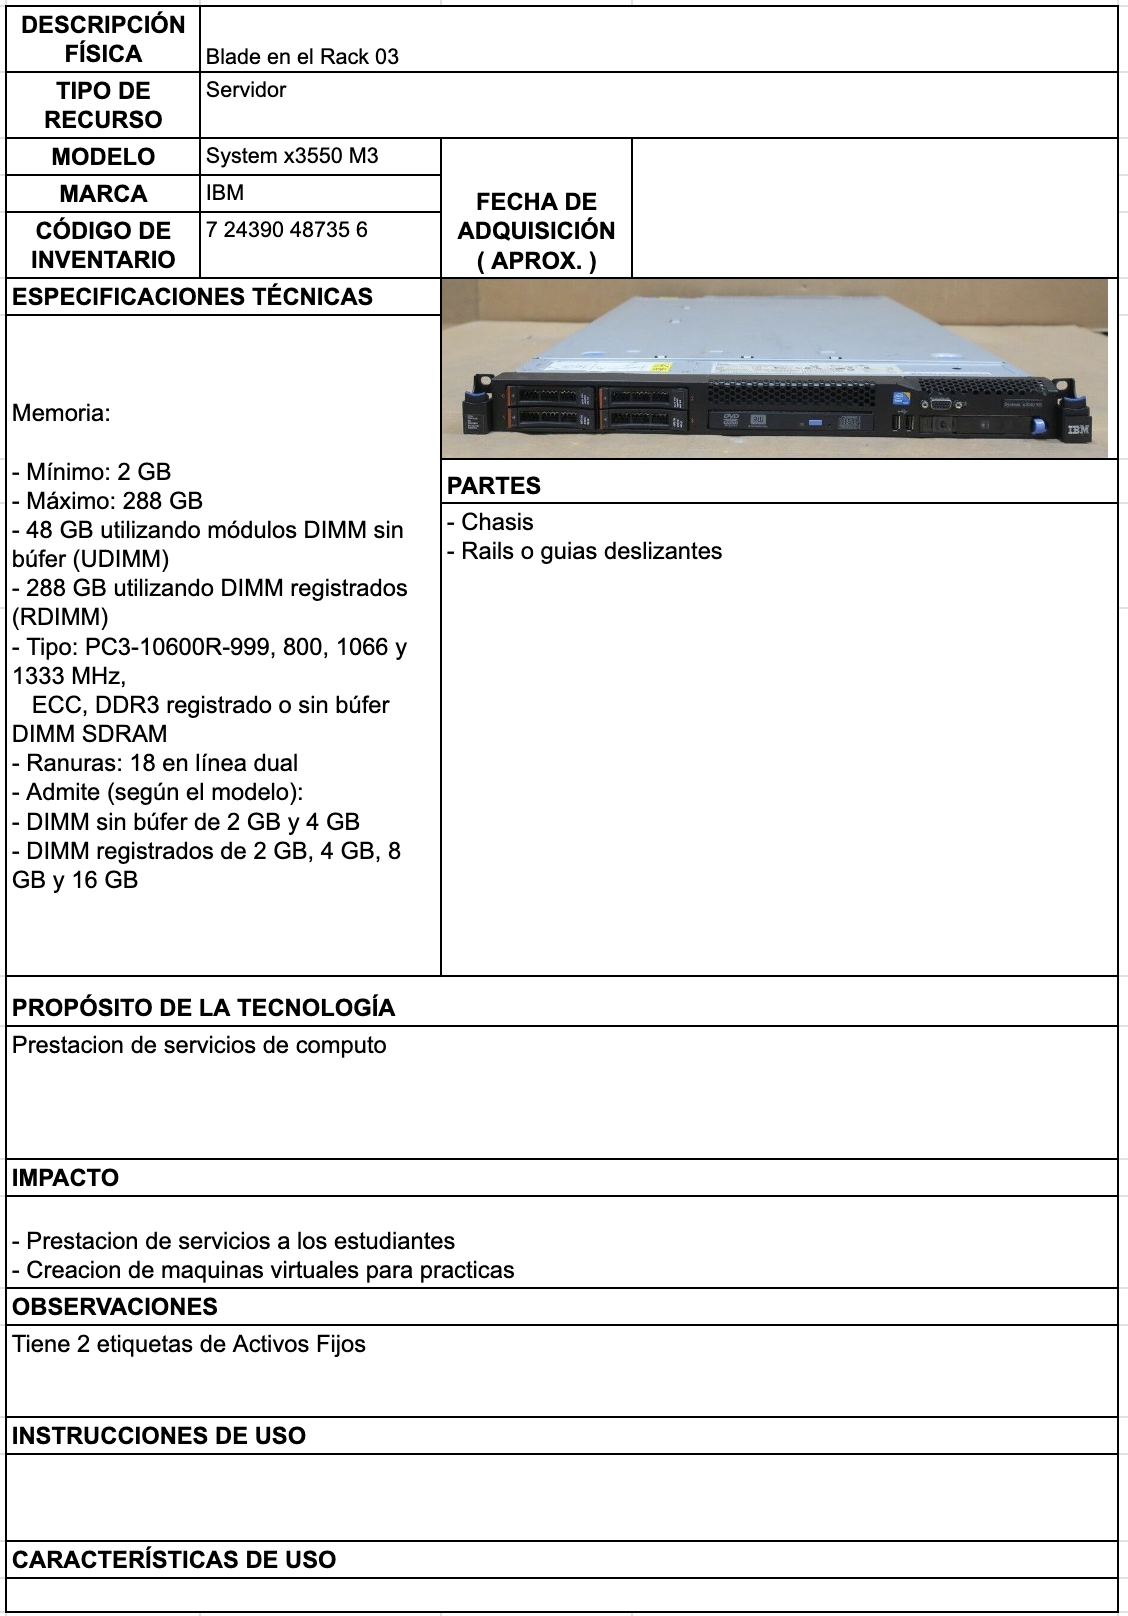
\includegraphics[width=0.25\textwidth,height=4cm,keepaspectratio]{tablas-images/cp1/racks/rack-3.png}} \\ \cline{1-1}
\textbf{MODELO:} Por definir & \\ \cline{1-1}
\textbf{MARCA:} Por definir & \\ \cline{1-1}
\textbf{CÓDIGO DE INVENTARIO:} Por definir & \\ \cline{1-1}
\textbf{FECHA DE ADQUISICIÓN (APROX.):} & \\ \hline
\multicolumn{2}{|l|}{\textbf{ESPECIFICACIONES TÉCNICAS}} \\ \hline
\multicolumn{2}{|p{0.95\textwidth}|}{
\footnotesize
Especificaciones por definir según imagen adjunta
} \\ \hline
\multicolumn{2}{|l|}{\textbf{PROPÓSITO:} Por definir} \\ \hline
\multicolumn{2}{|l|}{\textbf{IMPACTO:} Por evaluar} \\ \hline
\multicolumn{2}{|l|}{\textbf{OBSERVACIONES:} Ver imagen para detalles} \\ \hline
\end{tabular}
\end{table}

% Rack 4
\begin{table}[H]
\centering
\caption{Ficha técnica -- Rack 4}
\label{tab:rack-4}
\begin{tabular}{|p{0.6\textwidth}|p{0.3\textwidth}|}
\hline
\multicolumn{2}{|l|}{\textbf{DESCRIPCIÓN FÍSICA:} Servidor tipo rack} \\ \hline
\textbf{TIPO DE RECURSO:} Rack & 
\multirow{5}{*}{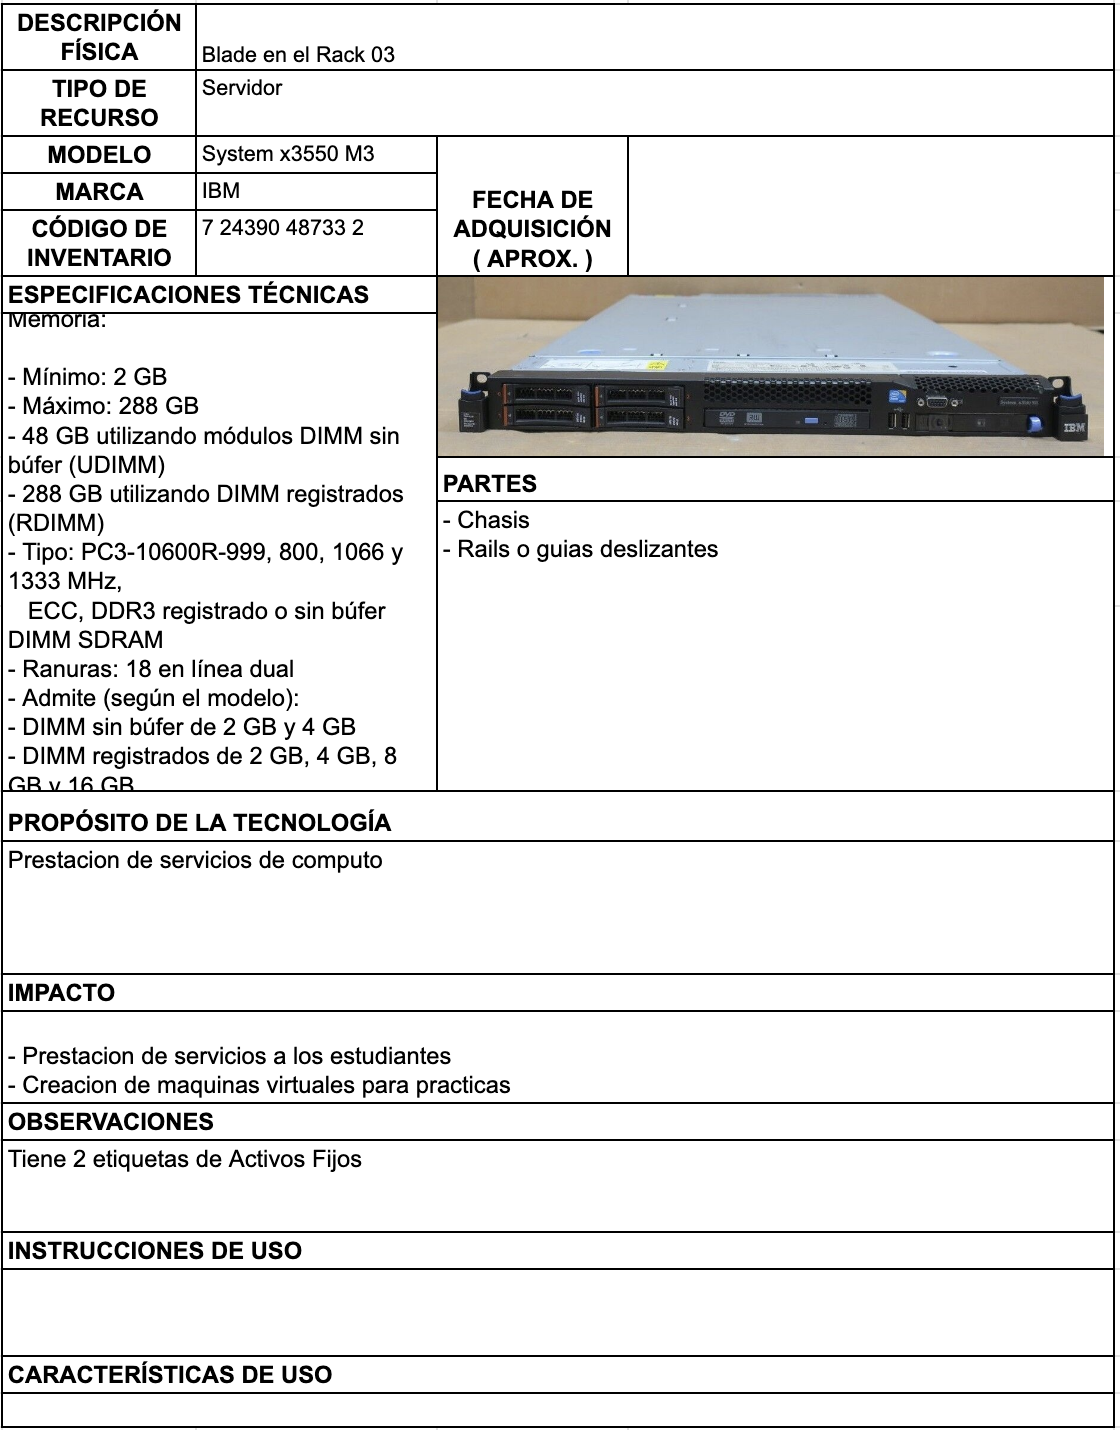
\includegraphics[width=0.25\textwidth,height=4cm,keepaspectratio]{tablas-images/cp1/racks/rack-4.png}} \\ \cline{1-1}
\textbf{MODELO:} Por definir & \\ \cline{1-1}
\textbf{MARCA:} Por definir & \\ \cline{1-1}
\textbf{CÓDIGO DE INVENTARIO:} Por definir & \\ \cline{1-1}
\textbf{FECHA DE ADQUISICIÓN (APROX.):} & \\ \hline
\multicolumn{2}{|l|}{\textbf{ESPECIFICACIONES TÉCNICAS}} \\ \hline
\multicolumn{2}{|p{0.95\textwidth}|}{
\footnotesize
Especificaciones por definir según imagen adjunta
} \\ \hline
\multicolumn{2}{|l|}{\textbf{PROPÓSITO:} Por definir} \\ \hline
\multicolumn{2}{|l|}{\textbf{IMPACTO:} Por evaluar} \\ \hline
\multicolumn{2}{|l|}{\textbf{OBSERVACIONES:} Ver imagen para detalles} \\ \hline
\end{tabular}
\end{table}

% Rack 5
\begin{table}[H]
\centering
\caption{Ficha técnica -- Rack 5}
\label{tab:rack-5}
\begin{tabular}{|p{0.6\textwidth}|p{0.3\textwidth}|}
\hline
\multicolumn{2}{|l|}{\textbf{DESCRIPCIÓN FÍSICA:} Servidor tipo rack} \\ \hline
\textbf{TIPO DE RECURSO:} Rack & 
\multirow{5}{*}{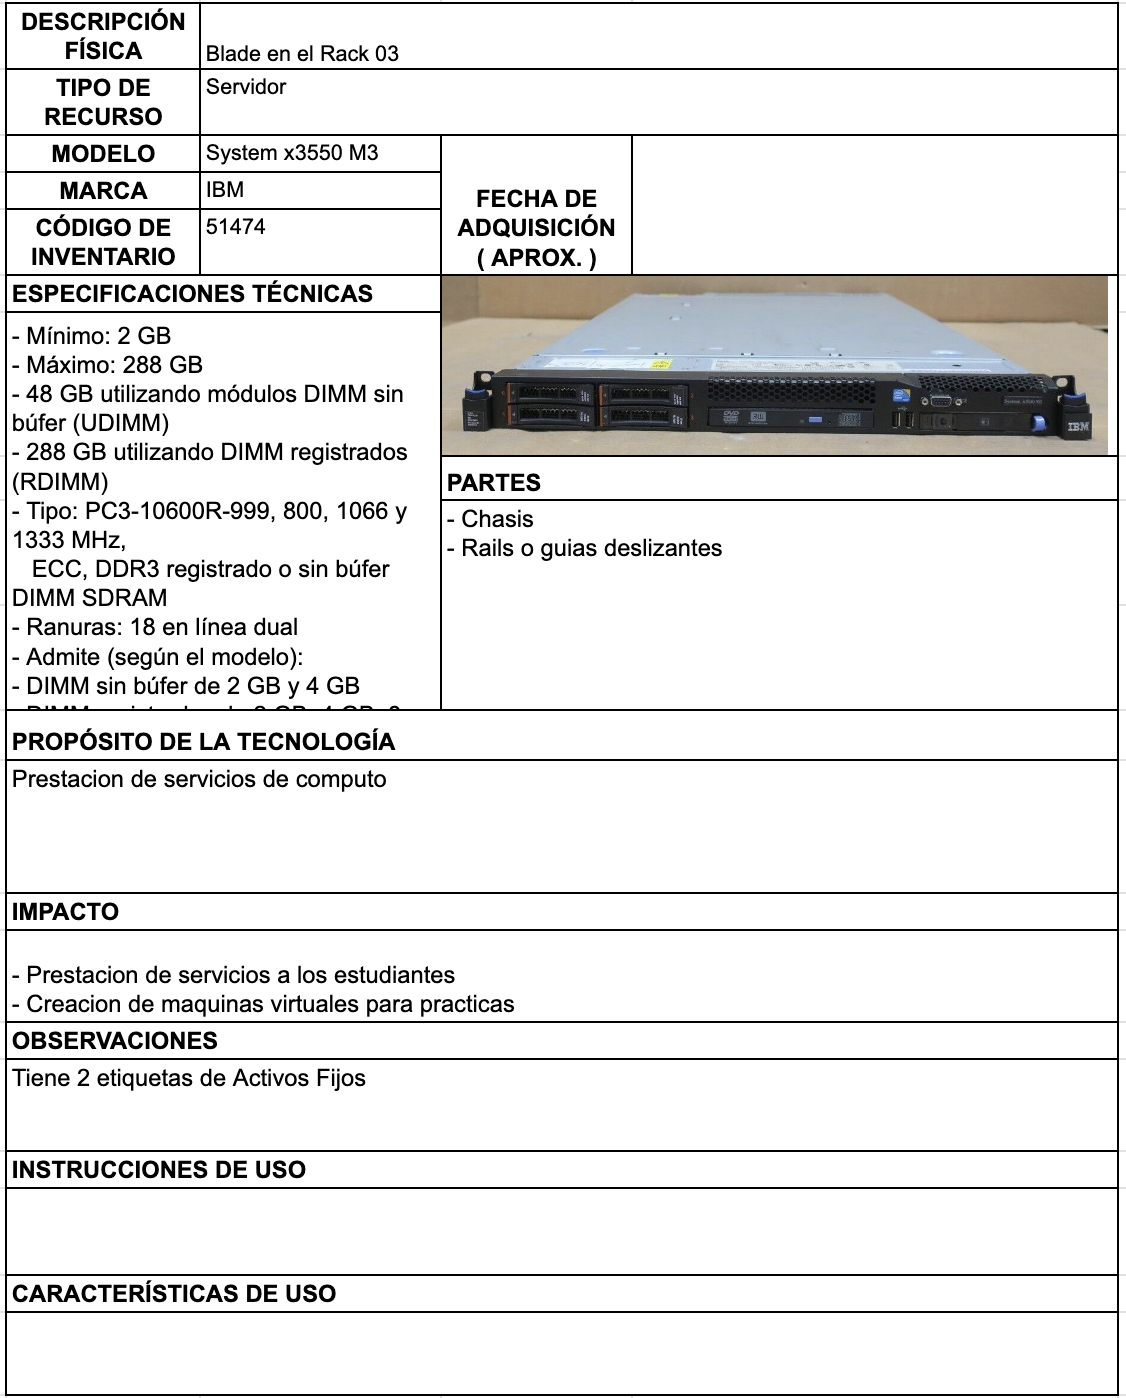
\includegraphics[width=0.25\textwidth,height=4cm,keepaspectratio]{tablas-images/cp1/racks/rack-5.png}} \\ \cline{1-1}
\textbf{MODELO:} Por definir & \\ \cline{1-1}
\textbf{MARCA:} Por definir & \\ \cline{1-1}
\textbf{CÓDIGO DE INVENTARIO:} Por definir & \\ \cline{1-1}
\textbf{FECHA DE ADQUISICIÓN (APROX.):} & \\ \hline
\multicolumn{2}{|l|}{\textbf{ESPECIFICACIONES TÉCNICAS}} \\ \hline
\multicolumn{2}{|p{0.95\textwidth}|}{
\footnotesize
Especificaciones por definir según imagen adjunta
} \\ \hline
\multicolumn{2}{|l|}{\textbf{PROPÓSITO:} Por definir} \\ \hline
\multicolumn{2}{|l|}{\textbf{IMPACTO:} Por evaluar} \\ \hline
\multicolumn{2}{|l|}{\textbf{OBSERVACIONES:} Ver imagen para detalles} \\ \hline
\end{tabular}
\end{table}

% NAS 1
\begin{table}[H]
\centering
\caption{Ficha técnica -- NAS 1}
\label{tab:nas-1}
\begin{tabular}{|p{0.6\textwidth}|p{0.3\textwidth}|}
\hline
\multicolumn{2}{|l|}{\textbf{DESCRIPCIÓN FÍSICA:} Sistema de almacenamiento conectado en red} \\ \hline
\textbf{TIPO DE RECURSO:} NAS (Network Attached Storage) & 
\multirow{5}{*}{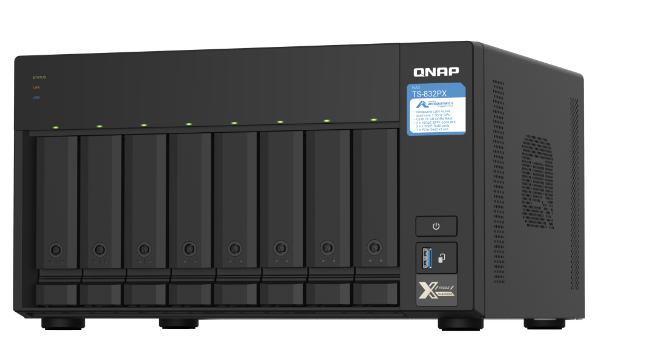
\includegraphics[width=0.25\textwidth,height=4cm,keepaspectratio]{tablas-images/cp1/NAS/nas-1.png}} \\ \cline{1-1}
\textbf{MODELO:} Por definir & \\ \cline{1-1}
\textbf{MARCA:} Por definir & \\ \cline{1-1}
\textbf{CÓDIGO DE INVENTARIO:} Por definir & \\ \cline{1-1}
\textbf{FECHA DE ADQUISICIÓN (APROX.):} & \\ \hline
\multicolumn{2}{|l|}{\textbf{ESPECIFICACIONES TÉCNICAS}} \\ \hline
\multicolumn{2}{|p{0.95\textwidth}|}{
\footnotesize
Especificaciones por definir según imagen adjunta
} \\ \hline
\multicolumn{2}{|l|}{\textbf{PROPÓSITO:} Por definir} \\ \hline
\multicolumn{2}{|l|}{\textbf{IMPACTO:} Por evaluar} \\ \hline
\multicolumn{2}{|l|}{\textbf{OBSERVACIONES:} Ver imagen para detalles} \\ \hline
\end{tabular}
\end{table}

% Firewall 1
\begin{table}[H]
\centering
\caption{Ficha técnica -- Firewall 1}
\label{tab:firewall-1}
\begin{tabular}{|p{0.6\textwidth}|p{0.3\textwidth}|}
\hline
\multicolumn{2}{|l|}{\textbf{DESCRIPCIÓN FÍSICA:} Sistema de seguridad de red} \\ \hline
\textbf{TIPO DE RECURSO:} Firewall & 
\multirow{5}{*}{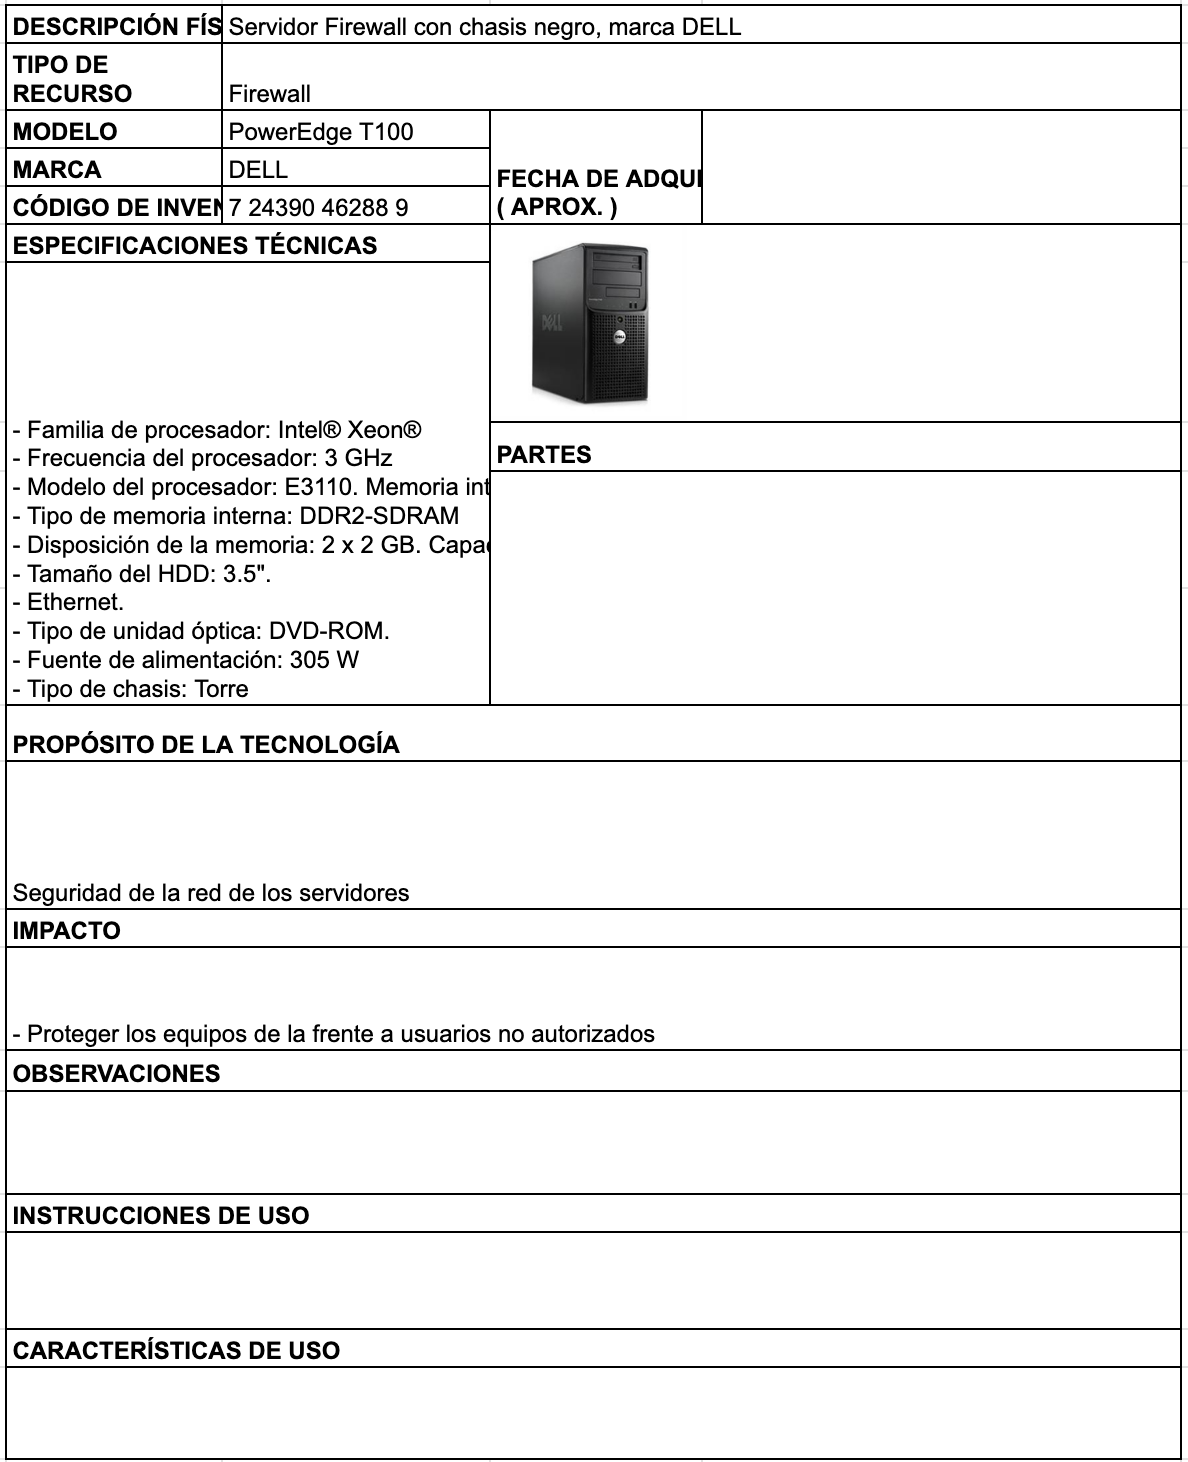
\includegraphics[width=0.25\textwidth,height=4cm,keepaspectratio]{tablas-images/cp1/firewall/firewall.png}} \\ \cline{1-1}
\textbf{MODELO:} Por definir & \\ \cline{1-1}
\textbf{MARCA:} Por definir & \\ \cline{1-1}
\textbf{CÓDIGO DE INVENTARIO:} Por definir & \\ \cline{1-1}
\textbf{FECHA DE ADQUISICIÓN (APROX.):} & \\ \hline
\multicolumn{2}{|l|}{\textbf{ESPECIFICACIONES TÉCNICAS}} \\ \hline
\multicolumn{2}{|p{0.95\textwidth}|}{
\footnotesize
Especificaciones por definir según imagen adjunta
} \\ \hline
\multicolumn{2}{|l|}{\textbf{PROPÓSITO:} Por definir} \\ \hline
\multicolumn{2}{|l|}{\textbf{IMPACTO:} Por evaluar} \\ \hline
\multicolumn{2}{|l|}{\textbf{OBSERVACIONES:} Ver imagen para detalles} \\ \hline
\end{tabular}
\end{table}

\section{Caracterización de servicios del GRID}
El \GRID\ ofrece una variedad de servicios tecnológicos a la comunidad académica, especialmente a los estudiantes de Ingeniería de Sistemas y Computación. Estos servicios incluyen:

\subsection{Servicios actuales}
Los servicios actuales del GRID se centran en la provisión de infraestructura de \TI\, incluyendo máquinas virtuales, almacenamiento y redes. Estos servicios son utilizados principalmente por estudiantes y docentes, los cuales se especifican en el cuadro~\ref{tab:servicios}.

\begin{table}[H]
\centering
\renewcommand{\arraystretch}{1.2}
\setlength{\tabcolsep}{3pt}
\tiny
\begin{tabularx}{\textwidth}{|>{\raggedright\arraybackslash}p{0.25\textwidth}|X|}
\hline
\textbf{NOMBRE DEL SERVICIO} & Máquinas Virtuales para estudiantes y docentes \\
\hline
\textbf{TIPO DE SERVICIO} & Servicio educativo \\
\hline
\textbf{PROPÓSITO} & Proveer máquinas virtuales a profesores, estudiantes y administrativos para prácticas académicas mediante XCP-ng. \\
\hline
\textbf{HORARIO DISPONIBILIDAD} & 24/7 \\
\hline
\textbf{TIEMPO FUNCIONAMIENTO} & 3 años \\
\hline
\textbf{RECURSOS} & Servidores torre y rack \\
\hline
\textbf{TECNOLOGÍAS} & Hipervisor tipo I (XCP-ng) \\
\hline
\textbf{IMPACTO} & Indisponibilidad afecta actividades misionales del grupo de investigación y programa de Ingeniería de sistemas. \\
\hline
\end{tabularx}
\caption{Caracterización de los servicios actuales del GRID}
\end{table}

\subsection{Servicios esperados}
Los servicios esperados por el GRID se orientan al aprovisionamiento de contenedores a traves de tecnologias VBC. Se espera que los usuarios de distintos dominios ( educación, investigación, extensión ) puedan beneficiarse de este nuevo servicio que se especifica en el cuadro ~\ref{tab:servicios-nuevos}

\begin{table}[H]
\centering
\renewcommand{\arraystretch}{1.2}
\setlength{\tabcolsep}{3pt}
\tiny
\begin{tabularx}{\textwidth}{|>{\raggedright\arraybackslash}p{0.25\textwidth}|X|}
\hline
\textbf{NOMBRE DEL SERVICIO} & Ambientes computacionales basados en \VBC\\
\hline
\textbf{TIPO DE SERVICIO} & Servicio de educación, investigación y extensión \\
\hline
\textbf{PROPÓSITO} & Proveer ambientes computacionales mediante tecnologías \VBC\ y mecanismo de orquestación \\
\hline
\textbf{HORARIO DISPONIBILIDAD} & 24/7 \\
\hline
\textbf{RECURSOS} & Servidores torre y rack \\
\hline
\textbf{TECNOLOGÍAS} & Por determinar \\
\hline
\textbf{IMPACTO} & Indisponibilidad afecta actividades misionales del grupo de investigación y programa de Ingeniería de sistemas. \\
\hline
\end{tabularx}
\caption{Caracterización de los servicios esperados del GRID}
\end{table}

\section{Descripción de la oportunidad}

Actualmente el Grupo de Investigación en Redes, Información y Distribución (\GRID) presenta diversas necesidades y oportunidades con relación a los servicios tecnológicos que ofrece a la Universidad del Quindío, en apoyo a sus objetivos misionales de docencia, investigación y extensión.

En este contexto, el \GRID\ busca identificar tecnologías emergentes que permitan potenciar su capacidad de brindar servicios tecnológicos avanzados, tanto para su propio beneficio como para la comunidad académica dentro de su ámbito de influencia.

Con relación a lo anterior, las \textbf{tecnologías de virtualización basadas en procesos} se presentan como una alternativa para optimizar la gestión de recursos y servicios de tecnología informática (\TI). Aunque el \GRID\ cuenta con una infraestructura basada en máquinas virtuales, gestionadas mediante el hipervisor tipo I XCP-ng, además de iniciativas de computación \textit{Desktop Cloud}, aún requiere de instancias computacionales más livianas para ampliar su oferta de servicios computacionales dirigidos a la comunidad académica, especialmente a los estudiantes del programa de Ingeniería de Sistemas y Computación de la Universidad del Quindío.

Como mencionan \textit{Sepúlveda et al.} (2022), las tecnologías de virtualización han proliferado en los últimos años y constituyen la base subyacente de infraestructuras modernas como el \textit{cloud computing}. A partir de esta proliferación, las Tecnologías de Virtualización Basadas en Contenedores (\VBC) se presentan como una alternativa que podría potenciar la gestión de los recursos relacionados con la infraestructura de \TI\ del \GRID.

Las tecnologías de \VBC\ representan una opción de virtualización que requiere menos recursos computacionales para su operación \citep{Xavier2013}, y que, en conjunto con las máquinas virtuales ya existentes en el \GRID\, podrían constituir una oferta de servicios de \TI\ con mayor diversificación, escalabilidad, flexibilidad y mantenibilidad, para satisfacer los requerimientos del contexto académico del grupo de investigación.

\section{Resumen de la entrevista con el cliente}

Para comprender mejor las necesidades y expectativas del \GRID\, se realizó una entrevista con el cliente.

\begin{itemize}
  \item \textbf{Entrevistado:} Luis Eduardo Sepúlveda Rodríguez
  \item \textbf{Fecha:} 6 de febrero de 2025
  \item \textbf{Duración:} 25 minutos
  \item \textbf{Link:} \href{https://drive.google.com/file/d/1rIc9xOsyDqumlTV-QXcw0inPyIbSEHLz/view?usp=sharing}{click aquí}
  \item \textbf{Asistentes:} Anubis Haxard Correa Urbano, José Alejandro Arias Pinzón
\end{itemize}

\subsection{Misión del grupo \GRID}
En el minuto 1:01 se menciona que: el grupo de investigación no declara una misión y visión distinta a la de su organización, la Universidad del Quindío. En consecuencia, estos elementos se heredan directamente de la institución.

\subsection{Actividades del grupo de investigación}
En el minuto 1:10 se menciona que: Aunque su nombre podría llevar al sesgo de pensar que se dedica exclusivamente a la investigación, el \GRID se desarrolla en los tres pilares misionales: docencia, investigación y extensión. Participa en actividades académicas como la enseñanza en el programa de Ingeniería de Sistemas y Computación, desarrolla investigaciones mediante el método científico, y realiza actividades de proyección social y formación complementaria.

\subsection{La virtualización basada en contenedores como una oportunidad}
En el minuto 3:01 se menciona que: Las tecnologías de \VBC pueden aportar al cumplimiento de la misión institucional. Actualmente se utiliza Docker por ser un estándar de facto, no por una evaluación formal. Existen alternativas como Podman, ContainerD y LXC que también podrían apoyar los tres pilares institucionales.

\subsection{El problema de la multitud de herramientas}
En el minuto 3:44 se menciona que: Existen muchas herramientas que podrían cumplir los objetivos institucionales. Escoger una tecnología adecuada no es trivial y requiere comprender el contexto organizacional. Por eso, este proyecto busca ofrecer una solución arquitectónica basada en \VBC\, que sirva a estudiantes y docentes para comprender el estado y las tendencias de estas tecnologías.

\subsection{Difusión para apoyar a otros grupos e instituciones}
En el minuto 5:32 se menciona que: Aunque el proyecto se enmarca en el \GRID\, sus resultados podrían ser útiles para otras universidades, grupos de investigación o incluso la industria. Elegir tecnologías \VBC\@estratégicamente puede tener gran valor, por lo que se plantea la necesidad de difundir los avances y resultados del proyecto.

\subsection{Restricción en los recursos}
En el minuto 7:08 se menciona que: El \GRID\ cuenta con infraestructura de \TI\, pero debe considerar su contexto y limitaciones. Soluciones que requieran licencias costosas o hardware especializado no son viables. Por tanto, las opciones de código abierto cobran especial relevancia.

\subsection{Impacto del proyecto en los campos de estudio del \GRID}
En el minuto 14:50 se menciona que: Los pilares misionales abarcan muchas actividades. El \GRID se enfoca en áreas como desarrollo de software, pensamiento computacional, computación paralela, análisis de datos, inteligencia artificial, redes, infraestructura de \TI, y HPC.\@Este proyecto busca fortalecer esas áreas mediante el uso de tecnologías \VBC.\@

\subsection{Necesidad de orquestación entre máquinas virtuales y contenedores}
Fuera del audio se menciona que: Actualmente los servicios se ejecutan sobre máquinas virtuales con XCP-ng. Se considera deseable —aunque no obligatorio— que la solución propuesta permita integrar contenedores con máquinas virtuales completas mediante un clúster, para maximizar el aprovechamiento de la infraestructura existente.

\bigskip\noindent \textit{Nota:} Este documento es solo un resumen de la entrevista. El audio incluye una explicación adicional del mapeo SMS que no se encuentra transcrita aquí.